
The model has been implemented in an iterative way. Function for
function, requirement for requirement. This process is very easy with
the use of QuickCheck.  In the beginning there were alot of negative
testing, because we didn't care about tweaking the generators.
By limiting the state space for negative tests, we achieved a better
ratio for positive testing when generating random tests. This was done
by letting some command sequences weight more than others when
QuickCheck generates the test cases. In
figure~\ref{QUICKCHECK:TWEAKING} we show how the state space is
minimized when QuickCheck has been tweaked.

\begin{figure}[!ht]
  \begin{center}
    \begin{minipage}[b]{0.6\linewidth}
      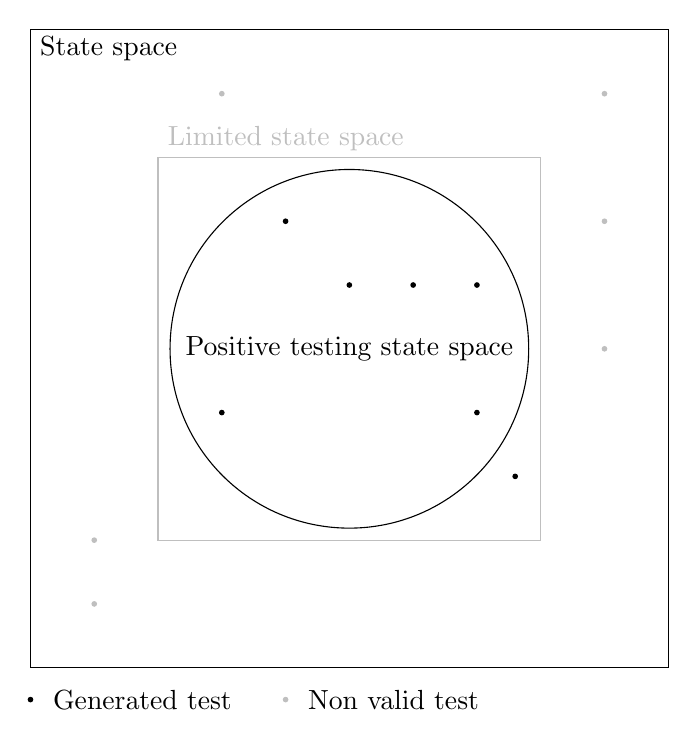
\begin{tikzpicture}[scale=0.81,
  valid/.style={fill=black},
  unvalid/.style={fill=black!25, color=black!25}]
\draw (0,0) rectangle (10,10) node [below, right] at
(0,9.7) {State space};
\draw [color=black!25] (2,2) rectangle (8,8) node [above, right] at
(2,8.3) {Limited state space};
\draw (5, 5) circle (80pt) node at (5,5) {Positive testing state space};

\draw [unvalid] (1,1) circle (1pt);
\draw [unvalid] (1,2) circle (1pt);
\draw [valid] (3,4) circle (1pt);
\draw [unvalid] (3,9) circle (1pt);
\draw [unvalid] (9,5) circle (1pt);
\draw [unvalid] (9,9) circle (1pt);
\draw [valid] (7,6) circle (1pt);
\draw [unvalid] (9,7) circle (1pt);
\draw [valid] (5,6) circle (1pt);
\draw [valid] (4,7) circle (1pt);
\draw [valid] (6,6) circle (1pt);
\draw [valid] (7,4) circle (1pt);
\draw [valid] (7.6,3) circle (1pt);

\draw [valid] (0,-0.5) circle (1pt) node [right] at (0.2,-0.5)
{Generated test};
\draw [unvalid] (4,-0.5) circle (1pt) node [right, color=black] at (4.2,-0.5)
{Non valid test};
\end{tikzpicture}
    \end{minipage}
  \end{center}
  \caption{The state space when tweaking QuickCheck's generators.}
  \label{QUICKCHECK:TWEAKING}
\end{figure}
The outer box in figure~\ref{QUICKCHECK:TWEAKING} represents the full
state space, and the inner circle represents positive test cases. This
means that all test cases outside of the circle represents negative
test cases. When tweaking generators it mean we can limit some of the
negative test state space, in order to have QuickCheck generate more
interesting positive test cases. The black dots in the figure
represents different generated test cases, and the gray dots
represents test cases which will not be generated after the new
limitations.

As an example, it is unnecessary to test functions if the watchdog
manager state machine has not been initialized with a call to the
\lstinline!WdgM_Init! function. We can weight the generation
of the \lstinline!WdgM_Init! function to be called with a higher ratio
if the state machine is not initialized yet.

\begin{lstlisting}[style=erlang, literate={_}{\_}1]
weight(S,  'WdgM_Init') ->
  case S#state.initialized of
    true                           -> 1;
    _                              -> 200
  end;
\end{lstlisting}

We want to do this because there is only some functions that actually
changes the state of the watchdog manager; there is a lot of so called
get-functions which only retrieves information.

Sometimes the model needs to be corrected because of ambiguities in
AUTOSAR or errors in the model. Quite often it was the C-code that had
the errors and needed to be corrected.  Easier when you do white box
testing, when the source code is known, because then you can really
check the code and compare with the requirements.

The C-code coverage was measured differently from the Erlang code
coverage, which used line coverage instead of condition/decision
coverage. Recursion is often used in functional programming languages
as Erlang, therefore it is not as suited for condition/decision
coverage as C-code is. Erlang also comes with a coverage library,
which makes it easy to use. On the other hand, measuring line coverage
in a imperative language like C is a bit redundant since statements
are executed sequentially. Therefore conditions/decision coverage
seems more reasonable.

We achieved fair coverage of the C-code, around 85\%, and the Erlang
code, around 97\%. The problem was the requirements, where we achieved
around 50\%. It would help if a QuickCheck model was implemented for
the whole system as well. Many of the requirements had dependencies in
other modules, and some requirements for the file structure, the
configuration or even the generation of files.

QuickCheck is good for overall testing, and can help with raising the
functional safety of modules.

%% analys av resultat
%% - coverage på modell och c-kod genom cover (erlang) och bullseye (c-kod)
%% - statistik på quickcheck körningar.

Stripped of comments and blank lines, the implemented Erlang model is
almost 1300 lines of code. This is to be compared with the C-code
which is over 14500 lines of code.
%% cat src/* inc/* generated_cfg/*.[c,h] stub/* rte/* gcc/* | grep -vP
%% ^[[:space:]]?'/\*' | grep -vP ^[[:space:]]?'\*' | grep -vP
%% ^[[:space:]]?'\\\*' | grep -v ^[[:space:]]$ | wc -l


\section{Future work}
An interesting thing we wanted to do from the beginning was to implementing
another module, preferably one that has some kind of dependency with the
watchdog manager. This is because then, it would be possible to testing towards
the phase ``system integration and testing'' in ISO~26262 and get even better
results.

Another good idea is to do more negative testing, and testing of null
pointers. This should be done to raise the coverage for the C-code to even
better levels.

We could also try new configurations. More configurations = better testing.
